\section{Validation and Accuracy}\label{sec:validation}

Establishing the reliability of the hybrid formulation requires verifying that its individual spherical and planar
modules reproduce exact analytical limits and quantifying the truncation error introduced by the dipolar closure. All
numerical results in this and the following sections are computed using \cref{alg:force} with the scripts listed in the
Data Availability Statement; unless stated otherwise, the dimensionless gap is set to $\varepsilon=1$, the Brinkman
viscosity ratios are $\mu_s/\mu=\mu_p/\mu=1$, and the interfacial slip and shell stress-jump parameters vanish
($\hat\ell_c=\beta_s=0$), as summarised in \cref{tab:params}. The impermeable no-slip sphere near a rigid wall
($\kappa=1$, $\alpha_p\to\infty$), studied by Zhang et al.~\cite{zhang2023unsteady}, serves as the baseline against which
the effects of substrate permeability and particle softness are measured.

In the absence of the wall, the particle solver is exact, as demonstrated in \cref{tab:validation}: it reproduces the
unsteady drag \eqref{eq:rigid_BC} of an impermeable sphere to all printed digits, matches the exact incident-flow
impedances \eqref{eq:rigid_Z}, and recovers the steady Debye--Bueche--Brinkman (DBB) drag ratio $\Omega=\hat
F_\infty/(-6\pi)$ of a homogeneous porous sphere~\cite{brinkman1949calculation} to within $10^{-4}$ at $\Wo=10^{-4}$, where
the residual reflects the $O(\Wo)$ unsteady correction. Likewise, the Fourier reflection module reproduces both limiting
substrate behaviours of \cref{sec:reflection}: in the transparent-interface limit ($\alpha_p=0$, $\beta_p=0$, $\mu_p=\mu$),
the computed interaction satisfies $|F_{\rm int}/F_\infty|<10^{-14}$, while a low-permeability layer with
$\alpha_p=10^5$ matches the rigid-wall reflection matrix to four significant digits. Every computed configuration is also
physically admissible: the wall-induced damping $\hat\gamma_{\rm int}$ remains strictly positive across all spectra
reported below (with a minimum of $0.035$), and the total damping $-\operatorname{Re}(F/U)$ is positive throughout,
including for positive stress jumps (\cref{app:checks}).

\begin{table}[t]
\caption{Parameters of the computations.}
\label{tab:params}
\begin{ruledtabular}
\begin{tabular}{lll}
Quantity & Values & Used in\\
\hline
$\Wo$ & $0.05$--$50$ (46 log-spaced values) & \cref{fig:spectra,fig:soft}\\
$\varepsilon$ & $0.25$--$5$ & \cref{fig:validation,fig:steady,fig:acoustic}\\
$\alpha_p$ & $3$--$100$ (11 log-spaced); $5,10,20,50,\infty$ & \cref{fig:woc_ap,fig:spectra}\\
$\beta_p$ & $-0.5,\ 0,\ 0.5$ & \cref{fig:woc_ap,fig:steady}\\
$\kappa$ & $0,\ 0.5,\ 0.7,\ 0.8,\ 0.95,\ 1$ & \cref{fig:soft}, \cref{tab:sensitivity}\\
$\alpha_s$ & $1$--$50$ & \cref{fig:soft}\\
CTC-like particle & $\kappa=0.9$, $\alpha_s=20$ & \cref{fig:acoustic}\\
leukocyte-like particle & $\kappa=0.7$, $\alpha_s=5$ & \cref{fig:acoustic}\\
\end{tabular}
\end{ruledtabular}
\end{table}

\begin{table}[t]
\caption{Validation. Top: unbounded fluid; $\hat F_\infty$ for an impermeable sphere at $\Wo=2$ against
\cref{eq:rigid_BC}, and the drag ratio $\Omega=\hat F_\infty/(-6\pi)$ of a homogeneous porous sphere at $\Wo=10^{-4}$
against the Debye--Bueche--Brinkman (DBB) formula. Bottom: steady ($\Wo\to0$) wall correction $F/F_\infty$ for an
impermeable sphere near a rigid wall.}
\label{tab:validation}
\begin{ruledtabular}
\begin{tabular}{lcc}
Case & Present & Reference\\
\hline
Impermeable, $\Wo=2$: $\hat F_\infty$ & $-45.5069+35.0349i$ & $-45.5069+35.0349i$\\
Porous, $\alpha_s=1$: $\Omega$ & $0.17561$ & $0.17561$ (DBB)\\
Porous, $\alpha_s=5$: $\Omega$ & $0.76342$ & $0.76338$ (DBB)\\
Porous, $\alpha_s=20$: $\Omega$ & $0.94669$ & $0.94663$ (DBB)\\
\hline
 & normal: present / Brenner~\cite{brenner1961slow} & parallel: present / Faxén series\\
$\varepsilon=0.5$ & $2.639$ / $3.205$ & $1.530$ / $1.615$\\
$\varepsilon=1$ & $2.018$ / $2.126$ & $1.365$ / $1.386$\\
$\varepsilon=2$ & $1.555$ / $1.569$ & $1.224$ / $1.227$\\
$\varepsilon=3$ & $1.377$ / $1.380$ & $1.161$ / $1.162$\\
$\varepsilon=4$ & $1.284$ / $1.285$ & $1.125$ / $1.126$\\
\end{tabular}
\end{ruledtabular}
\end{table}

Because the wall interaction neglects multipoles of order $l\ge2$, its accuracy is assessed at both ends of the
frequency spectrum in \cref{fig:validation}. In the steady limit ($\Wo\to0$) shown in \cref{fig:validation}(a) and
\cref{tab:validation}, where the bispherical-coordinate solution of Brenner~\cite{brenner1961slow} is exact, the dipolar
closure underestimates the normal wall correction by $5.1\%$ at $\varepsilon=1$, $0.9\%$ at $\varepsilon=2$, and less than
$0.3\%$ for $\varepsilon\ge3$, tracking the classical $O(x^3)$ reflection series closely for $\varepsilon\le4$ with a
residual of order $O(x^4)$ as anticipated in \cref{sec:closure}. Parallel oscillation is even more accurate, agreeing
with the $O(x^5)$ Faxén series to within $1.5\%$ at $\varepsilon=1$, because the leading neglected multipole coefficient
is smaller. At smaller clearances ($\varepsilon=0.5$), the normal-motion error grows to $18\%$, confirming that
near-contact lubrication requires higher multipoles; consequently, all quantitative results in the remainder of this paper
are restricted to $\varepsilon\ge1$. At the opposite, high-frequency end of the spectrum, \cref{fig:validation}(b) confirms
that the wall-induced added mass $m_{\rm int}/m_f$ at $\varepsilon=1$ decreases monotonically towards the leading inviscid
image values $3/(16h^3)=0.0234$ (normal) and $3/(32h^3)=0.0117$ (parallel) given by \cref{eq:inviscid}. At $\Wo=160$,
the computed values are $0.0246$ and $0.0122$, with the remaining $5\%$ difference arising from higher-order dipolar image
reflections retained by the closure and from $O(\Wo^{-1})$ viscous boundary layers. To verify that the neglected $l\ge2$
multipoles do not distort the finite-frequency crossovers at $\varepsilon=1$, we also performed an independent
axisymmetric finite-element method (FEM) check using Taylor--Hood elements for normal oscillation. The FEM benchmark
yields a rigid-wall crossover of $\Wo_c=3.04$ (compared with $2.92$ from the dipolar closure) and, for a permeable layer
with $\alpha_p=20$ and $\beta_p=0$, an upward crossover of $\Wo_c^{\uparrow}=3.15$ (against $3.06$), a damping of
$\hat\gamma_{\rm int}=0.280$ at $\Wo=3$ (against $0.281$), and a downward crossover of $\Wo_c^{\downarrow}=41.2$ (against
$46$), confirming that the dipolar closure faithfully captures both the force magnitudes and the crossover structure for
$\varepsilon\ge1$.

\begin{figure*}[t]
  \centering
  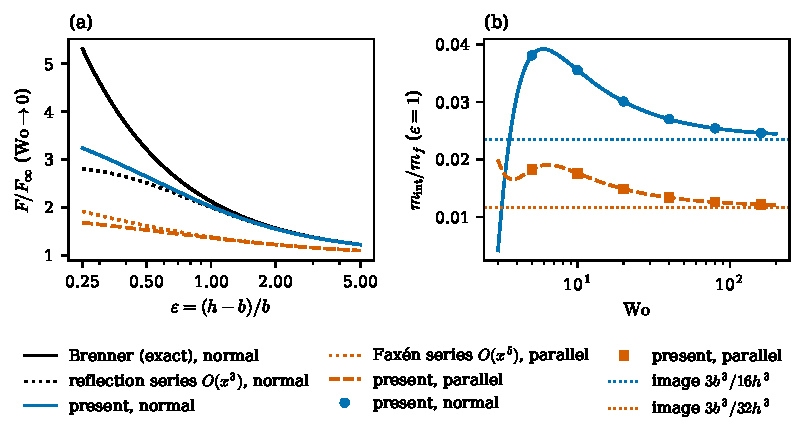
\includegraphics[width=\linewidth]{figures/fig2_validation.pdf}
  \caption{Validation for an impermeable sphere near a rigid wall. (a) Steady wall correction $F/F_\infty$ against the
  gap $\varepsilon$, compared with Brenner's exact solution~\cite{brenner1961slow} and the classical reflection series
  $1/(1-\tfrac98x+\tfrac12x^3)$, $x=b/h$ (normal), and with Faxén's series to $O(x^5)$ (parallel). (b) Wall-induced
  added mass $m_{\rm int}/m_f$ against $\Wo$ at $\varepsilon=1$, approaching the inviscid image values of
  \cref{eq:inviscid} (dotted); markers show the values tabulated in the text.}
  \label{fig:validation}
\end{figure*}
